%! Author = rikpe
%! Date = 24/04/2021

\section{Context Based Research}\label{sec:context-based-research}

%Leeruitkomst 2 - Contextgericht onderzoek Je onderbouwt je keuzes voor processen en technieken aan de hand van een
%algemeen geaccepteerde onderzoeksmethode en rekening houdend met je eigen ethische waarden.
%Verdere toelichting Je onderbouwt je keuzes voor processen en technieken aan de hand van contextgebaseerd onderzoek.
%Je maakt gebruik van bekende en algemeen geaccepteerde onderzoeksmethoden of -modellen, zoals het DOT Framework en
%ICT Research Methods.
%Je communiceert je onderzoeksaanpak, plan, resultaten en conclusie zowel mondeling als schriftelijk.

%Wat wil ik leren
Dit semester wil ik leren om doelgericht onderzoek te doen waarvan de uitkomsten kunnen bijdragen aan het ontwikkelen van technische en complexe software oplossingen.
Onderzoek is nodig om kennis op te doen bij een bepaald onderwerp en om deze zo beter te kunnen begrijpen.
Vanuit daar kun je je kennis stapsgewijs (onderzoek voor onderzoek) opbouwen om zo tot een gepaste oplossing te
komen voor een probleem.


%Wat moet ik doen om dit te kunnen bereiken? / %Welke middelen heb ik hiervoor nodig?
Door de onderzoeksmethodieken te gebruiken die in het DOT-framework staan omschreven kan ik doelgericht onderzoek
doen.
Voor het onderzoek ga ik verschillende methodieken combineren om zo tot een oplossing te komen op mijn probleem.


%Hoe ga ik success meetbaar maken?
Dit leerdoel ga ik meetbaar maken door onderzoeksdocumenten op te leveren die door zowel mij als door een ander als
nuttig worden beschouwd en daarmee ook een bijdrage kunnen leveren aan een oplossing van een complex probleem.
Ik definieer mijn kwaliteit op de feedback die ik heb ontvangen van vak bekwame experts "docenten".

%Wat heb ik gedaan om dit aan te tonen?
Bij zowel het groepsproject als het individueel project heb ik verschillende casestudies gemaakt die voor een klant
kunnen helpen bij het maken van een keuze om zo een probleem op te lossen.

\bigskip
\subsection{Ontwikkel process}
%evaluatie / %Beoordeling
\subsubsection{Case Studies}
\paragraph{Evaluatie: 24-04-2021}
Tijdens het groepsproject hebben we zes verschillende case studies moeten uitwerken.
Deze case studies gaven een complex probleem weer waar een oplossing bij gevonden moest worden.
De problemen deden zich voor op verschillende aspecten binnen het ontwikkelen van software.
De case studies zijn uitgewerkt door middel van het toepassen van verschillende methodieken uit het DOT-framework.
De casestudies die tijdens het proftaak groepje zijn behandeld, zijn goed afgerond en de feedback van de leraren is
verwerkt.
Daarom beschouw ik mijn huidige oriëntatie als "georiënteerd".
Deze case studies zijn terug te vinden in het canvas bij he opdrachtenoverzicht van project groep 3.
Bij de verschillende case studies hebben we taken verdeeld. Mijn bijdrage aan de case studies zijn als volgt:

\begin{itemize}
	\setlength{\itemsep}{0pt}%
	\setlength{\parskip}{0pt}%
	\item Gebrainstormd over de case studie; wat houdt deze in en wat vragen ze van ons
	\item Onderzoeksvragen opgesteld gebaseerd op de brainstorm sessie
	\item Onderbouwde feedback gegeven op elkaars uitwerking op een vraag en waar nodig ondersteund.
	\item Onderzoeksvragen en deelvragen uitgewerkt.

\end{itemize}

Gebaseerd op de feedback van onze docenten ligt onze kwaliteit hoog.
Alle feedback die we ontvangen wordt genotuleerd en wordt in de volgende case studie meegenomen.

\subsubsection{Onderzoek}
\paragraph{Evaluatie: 05-04-2021}
Voor het individuele project heb ik ook context based research toegepast voor het "cache van data binnen mijn project".
Ook tijdens dit onderzoek is het dot onderzoeks framework toegepast.
Uit het dot framework heb ik de volgende methodes uitgekozen:

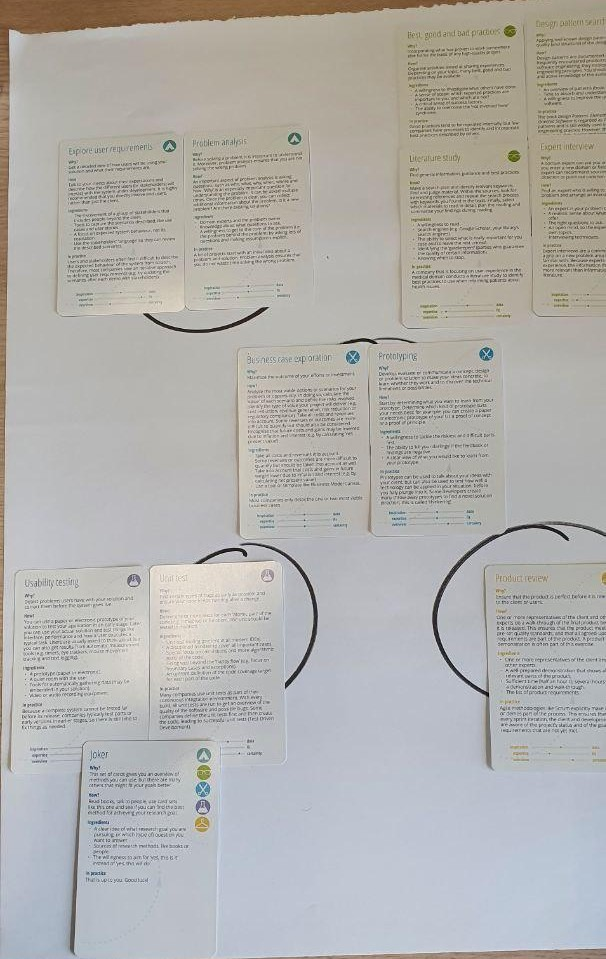
\includegraphics[width=\textwidth,height=\textheight,keepaspectratio]{Context_Based_Research_Defined_Research_Methodes.jpg}\label{fig:research_methodes}

Deze methodes zijn besproken met Tom Langhorst docent gespecialiseerd het contextueel onderzoeken.

De onderzoeks vraag luid als volgt: "Hoe wordt caching toegepast op enterprise software niveau voor specifieke doeleinde binnen het java framework springboot?"

Tijdens het onderzoek zijn de toepassingen van caching mijzelf zeer duidelijk geworden.
Bij het onderzoek hebben we ook enkelen prototypes gemaakt de de snelheid en de toepassing van caching goed laat zien.
Na het prototype hebben we aan een vak expert om feedback gevraagd tijdens dit feedback moment hebben we het over verschillende topics gehad bij komen kijken bij het cachen van data.

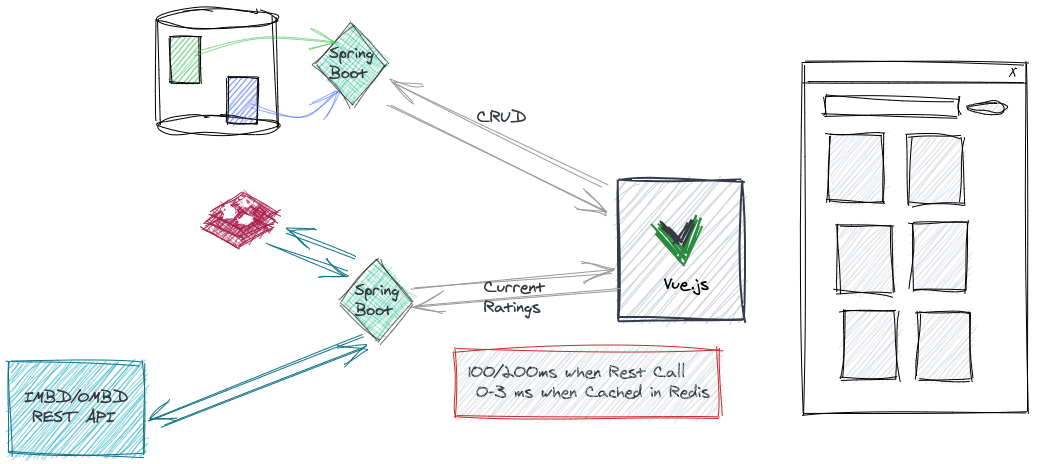
\includegraphics[width=\textwidth,height=\textheight,keepaspectratio]{Redis_Archtecture.png}\label{fig:redis_architecture}

\subsection{Eind beoordeling / reflectie}
Ik ontzetten veel geleerd over de contextueel onderzoek doen naar een topic en heb geleerd hoe ik een onderzoeksvraag moet samenstellen.
Gebaseerd op de verschillende case studies en groeps onderzoeken en het individueel onderzoek beschouw ik mijn huidige bekwaamheid tot dit leerdoel op:\\
\par\vspace{10pt}\textbf{\uppercase{"Proficient"}}\\


\newpage
